\documentclass[aspectratio=169]{beamer}
\usepackage{lmodern}
%\usetheme{Madrid}
%\usecolortheme{giantoak}
\newcommand*\oldmacro{}
\let\oldmacro\insertshorttitle
\renewcommand*\insertshorttitle{\oldmacro\hfill\insertframenumber\,/\,\inserttotalframenumber}
% \newcommand{\light}[1]{\textcolor{gray}{#1}}
%\usepackage{beamerthemesplit}
\usepackage{textpos}
\usepackage{pgf}
%\logo{\pgfputat{\pgfxy(0,-.4)}{\pgfbox[right,base]{\includegraphics[height=1.0cm]{logo.jpg}}}}
%\newcommand{\nologo}{\setbeamertemplate{logo}{}}
\usepackage{booktabs}
\usepackage{graphicx}
%\theoremstyle{principle}
%\newtheorem*{principle}{Design Principle}

\title{Logistic Regression}
%\author[Jeremy Kedziora]{\includegraphics[height=2.5cm]{logo.jpg}\\Jeremy Kedziora\\
%\small{Chief Scientist}\\
%\small{Giant Oak}}
\date{\today}

\begin{document}

{
%\nologo
\begin{frame}
    \maketitle
\end{frame}
}


%@@@@@@@@@@@@@@@@@@@@@@@@@@@@@@@@@@@@@@@@@@@@@@@@@@@@@@
\begin{frame}
\frametitle{Objectives}
\begin{itemize}
\item Understand Logistic Regression as a Generalized Linear Model;
\bigskip
\bigskip
\item Develop intuition for ideas behind Maximum Likelihood Estimation;
\bigskip
\bigskip
\item Build ability to interpret Logistic Regression results;
\end{itemize}
\end{frame}

%@@@@@@@@@@@@@@@@@@@@@@@@@@@@@@@@@@@@@@@@@@@@@@@@@@@@@@
\begin{frame}
\frametitle{Binary data}
We have learned about and worked with linear regression:
\bigskip
\begin{itemize}
\item model parameter interpretation;
\bigskip
\item hypothesis tests and p-values;
\bigskip
\item model fit, e.g. residuals.
\bigskip
\end{itemize}
This is great when the dependent variable is \textbf{continuous} (i.e. interval or ratio data).\\
\bigskip
\onslide<2->But what if the dependent variable is \textbf{weird}, e.g. binary?
\end{frame}

%@@@@@@@@@@@@@@@@@@@@@@@@@@@@@@@@@@@@@@@@@@@@@@@@@@@@@@
\begin{frame}
\frametitle{Binary data}
\begin{center}
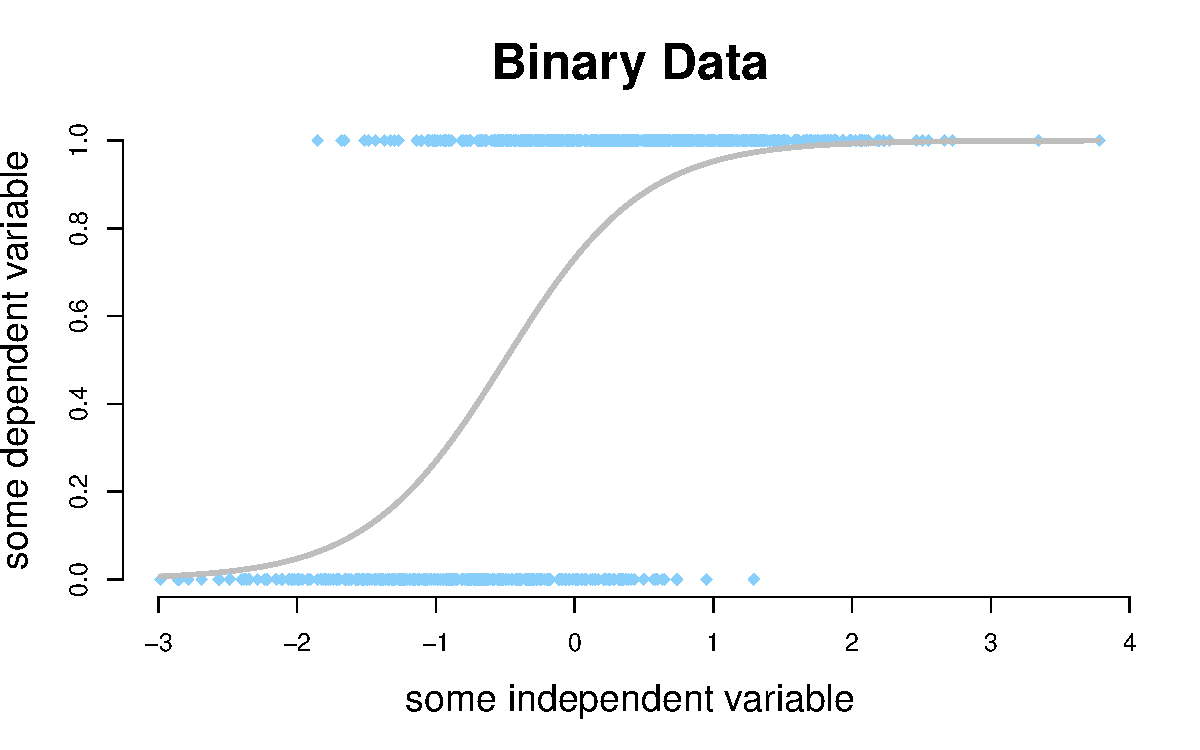
\includegraphics[scale=0.55]{binary_data_w_s_curve.pdf}
\end{center}
\end{frame}

%@@@@@@@@@@@@@@@@@@@@@@@@@@@@@@@@@@@@@@@@@@@@@@@@@@@@@@
\begin{frame}
\frametitle{A specific example...}
\begin{columns}

\begin{column}{0.5\textwidth}
After colliding with an iceberg late on 14 April 1912 RMS \textit{Titanic} sank with huge loss of life:
\bigskip
\begin{itemize}
\item Estimated that 2,224 passengers and crew were aboard;
\bigskip
\item Carried 20 lifeboats with sufficient capacity for 1,178;
\bigskip
\item<2-> Even with perfect efficiency 1,046 people were doomed.
\bigskip
\end{itemize}

\end{column}

\onslide<1->
\begin{column}{0.5\textwidth}  %%<--- here
    \begin{center}
     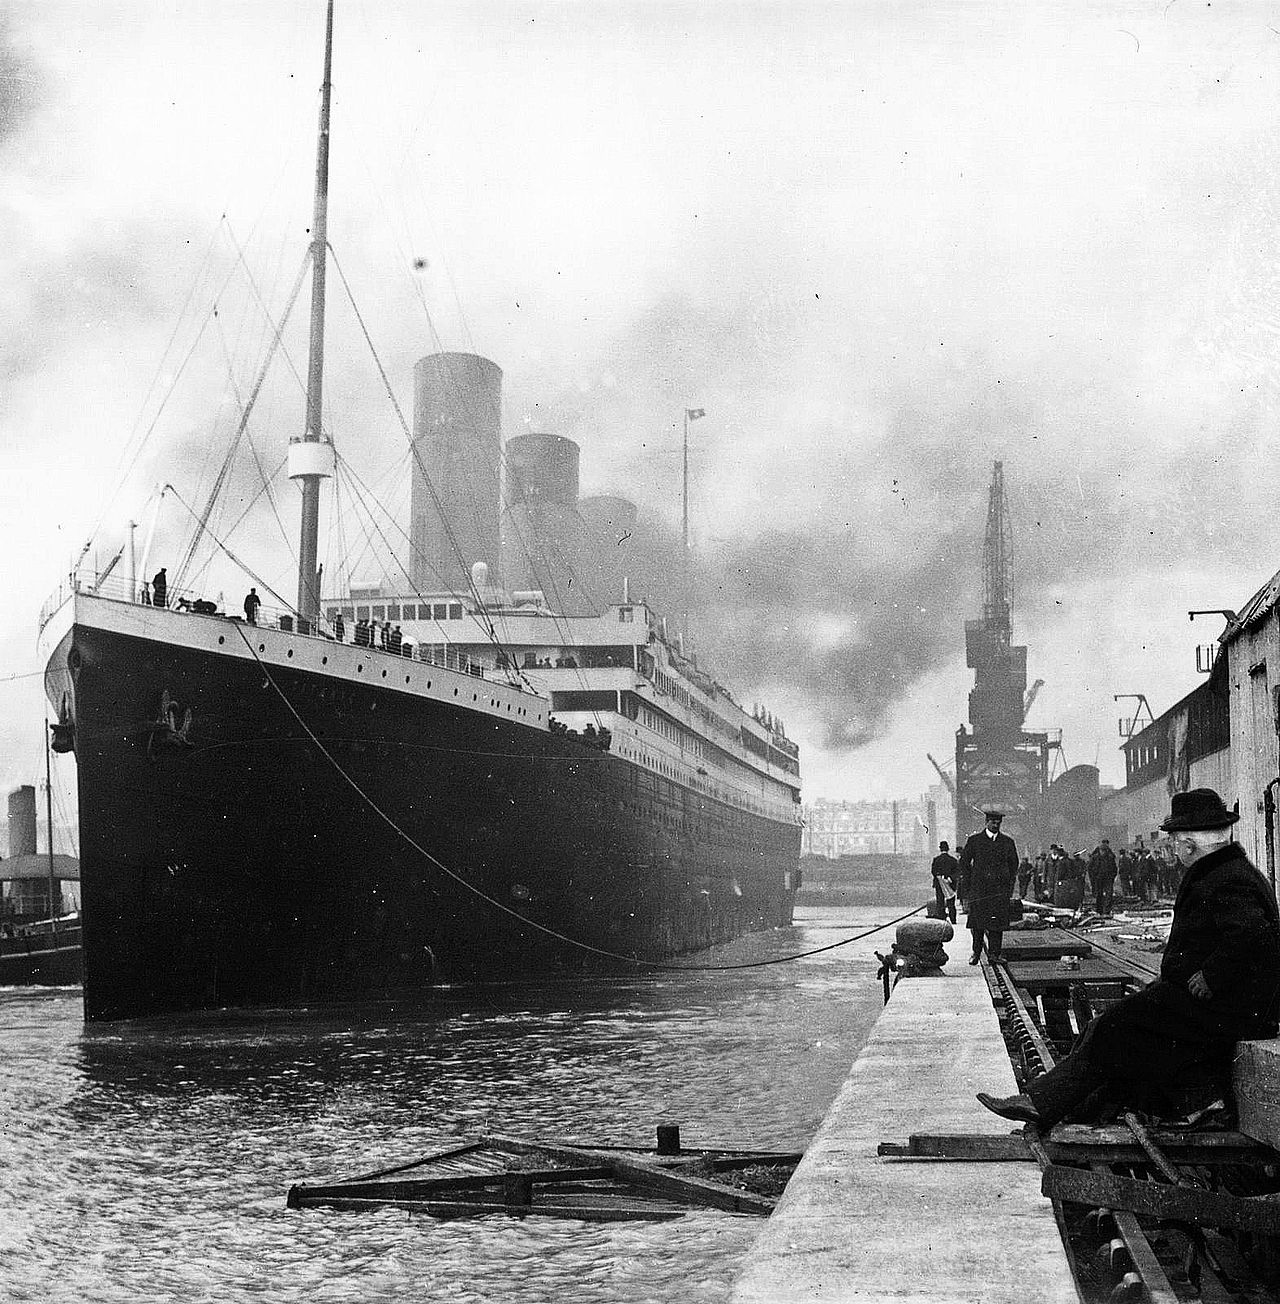
\includegraphics[scale=0.12]{1280px-Titanic.jpg}
     \end{center}
\end{column}

\end{columns}
\end{frame}

%@@@@@@@@@@@@@@@@@@@@@@@@@@@@@@@@@@@@@@@@@@@@@@@@@@@@@@
\begin{frame}
\frametitle{A specific example... who lived and who died?}


\begin{columns}

\begin{column}{0.5\textwidth}

\begin{center}
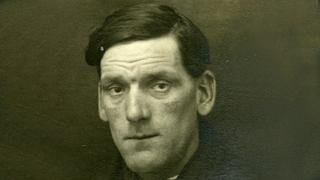
\includegraphics[scale=0.55]{_59403930_john_priest_landscape.jpg}
\end{center}

\begin{center}
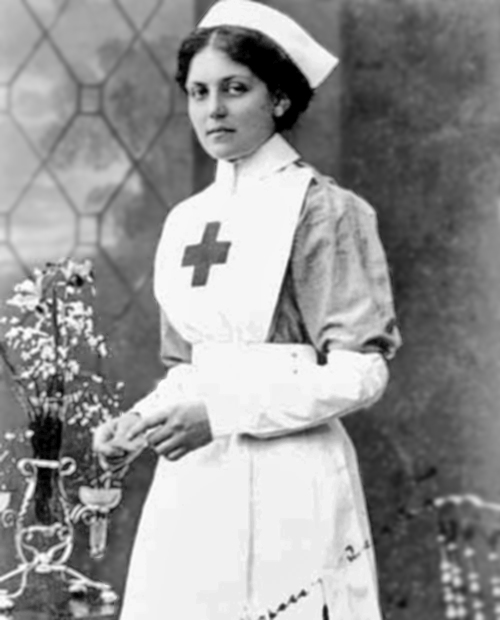
\includegraphics[scale=0.18]{Violet_jessop_titanic.jpg}
\end{center}

\end{column}

\begin{column}{0.5\textwidth}  %%<--- here

\begin{center}
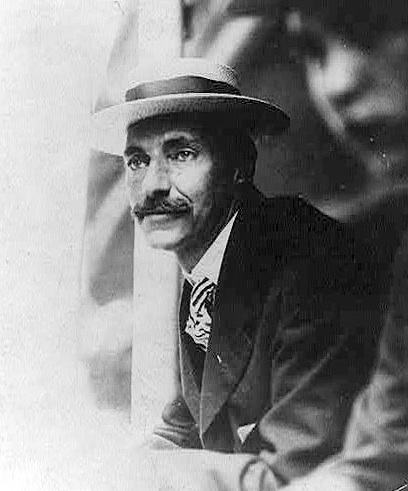
\includegraphics[scale=0.4]{John_Jacob_Astor_1909.jpg}
\end{center}

\end{column}

\end{columns}

\end{frame}

%@@@@@@@@@@@@@@@@@@@@@@@@@@@@@@@@@@@@@@@@@@@@@@@@@@@@@@
\begin{frame}
\frametitle{A specific example... who lived and who died?}

\begin{table}
\begin{tabular}{r | c | c | c | c | c | c | c}
Survived & Pclass  & Name & Sex & Age & Siblings & Parents & Fare\\
 &   &  &  &  & Spouses & Children & \\
\hline \hline
0 & 3 & Owen Harris Braund &M&22&1&0&7.25\\ 
 1 & 1 & Mrs. John Cumings &F&38&1&0&71.28\\ 
  1 & 3 & Miss. Laina Heikkinen &F&26&0&0&7.92\\ 
   1 & 1 & Mrs. Jacques Futrelle &F&35&1&0&53.10\\ 
   $\vdots$ & $\vdots$ & $\vdots$ &$\vdots$&$\vdots$&$\vdots$&$\vdots$&$\vdots$\\ 
%Norman P & 8:00 & 22:45 & 23:02 & 53:47 \onslide<4->\\
%Alex K & 14:00 & 28:00 & n/a & n/a \onslide<5->\\
%Sarah H & 9:22 & 21:10 & 24:03 & 54:35 
\end{tabular}
\end{table}

\end{frame}

%@@@@@@@@@@@@@@@@@@@@@@@@@@@@@@@@@@@@@@@@@@@@@@@@@@@@@@
\begin{frame}
\frametitle{Logistic Regression}

Logistic Regression (logit) is a Generalized Linear Model (GLM) used to model a binary dependent variable using numerical and categorical predictors.\\
\bigskip
\onslide<2-> Recall that GLMs have three required components:
\begin{enumerate}
\item A probability distribution that describes the dependent variable;
\item A linear model $\beta_0 + \beta_1x_1 + \beta_2x_2 + ...$;
\item A link function that relates the linear model to the dependent variable distribution.
\end{enumerate}

\end{frame}

%@@@@@@@@@@@@@@@@@@@@@@@@@@@@@@@@@@@@@@@@@@@@@@@@@@@@@@
\begin{frame}
\frametitle{A probability distribution that describes the dependent variable}

\begin{itemize}
\item For logit assume that for a given set of predictor variables (say $x$):
\begin{align*}
y &= 1 \mbox{ w/ probability }p(1)\\
y &= 0 \mbox{ w/ probability }1 - p(1);
\end{align*}
\bigskip
\item We want to model $p(1)$ and figure out how it depends on $x$.

\end{itemize}
\end{frame}

%@@@@@@@@@@@@@@@@@@@@@@@@@@@@@@@@@@@@@@@@@@@@@@@@@@@@@@
\begin{frame}
\frametitle{A linear model $\beta_0 + \beta_1x_1 + \beta_2x_2 + ...$}

\begin{itemize}
\item The $x$'s are independent variables that come from the data and are the input to logit;
\bigskip
\bigskip
\item The $\beta$'s are the effects of the independent variables and are the output of logit;
\bigskip
\bigskip
\item In the Titanic example, the $x$'s could be any of Pclass, Sex, Age, Siblings, Parents, and Fare.

\end{itemize}
\end{frame}

%@@@@@@@@@@@@@@@@@@@@@@@@@@@@@@@@@@@@@@@@@@@@@@@@@@@@@@
\begin{frame}
\frametitle{A link function that relates the linear model to the dependent variable distribution}

This is where the rubber meets the road...\\
\bigskip
Let's talk a little about \textbf{odds}:
\onslide<2->
\begin{itemize}
\item In the Titanic context we can ask \textbf{what are the odds that a passenger lives?}
\begin{align*}
Odds(\mbox{Lived}) = \frac{p(\mbox{Lived})}{p(\mbox{not Lived})} = \frac{p(\mbox{Lived})}{1 - p(\mbox{Lived})}.
\end{align*}
%\item The \textbf{Logit} of probability $p(\mbox{Died})$ is defined as the ln of the odds:
%\begin{align*}
%\mbox{Logit}(p(\mbox{Died})) = \mbox{ln}\left(\frac{p(\mbox{Died})}{1 - p(\mbox{Died})}\right).
%\end{align*}
\onslide<3->\item The \textbf{Logistic Function} is defined as the inverse of:
\begin{align*}
%p(\mbox{Lived}) = \frac{\exp\{\beta_0 + \beta_1x_1 + \beta_2x_2 + ...\}}{1 + \exp\{\beta_0 + \beta_1x_1 + \beta_2x_2 + ...\}}
 \ln\left(Odds(Lived)\right) = \ln\left(\frac{p(\mbox{Lived})}{1 - p(\mbox{Lived})}\right).
\end{align*}
\onslide<3->It is used because:
\begin{itemize}
\item[] %It takes the linear model and ensures that it will give us something between 0 and 1;
\item[] %It makes writing the odds of two events really easy.
\end{itemize}

\end{itemize}

\end{frame}



%@@@@@@@@@@@@@@@@@@@@@@@@@@@@@@@@@@@@@@@@@@@@@@@@@@@@@@
\begin{frame}
\frametitle{A link function that relates the linear model to the dependent variable distribution}

This is where the rubber meets the road...\\
\bigskip
Let's talk a little about \textbf{odds}:
\onslide<1->
\begin{itemize}
\item In the Titanic context we can ask \textbf{what are the odds that a passenger lives?}
\begin{align*}
Odds(\mbox{Lived}) = \frac{p(\mbox{Lived})}{p(\mbox{not Lived})} = \frac{p(\mbox{Lived})}{1 - p(\mbox{Lived})}.
\end{align*}
%\item The \textbf{Logit} of probability $p(\mbox{Died})$ is defined as the ln of the odds:
%\begin{align*}
%\mbox{Logit}(p(\mbox{Died})) = \mbox{ln}\left(\frac{p(\mbox{Died})}{1 - p(\mbox{Died})}\right).
%\end{align*}
\onslide<1->\item After some algebra for a number $\gamma$:
\begin{align*}
\mbox{Logistic}(\gamma) = \frac{\exp\{\gamma\}}{1 + \exp\{\gamma\}}.
\end{align*}
\onslide<1->It is used because:
\begin{itemize}
\item[] %It takes the linear model and ensures that it will give us something between 0 and 1;
\item[] %It makes writing the odds of two events really easy.
\end{itemize}

\end{itemize}

\end{frame}
%

%@@@@@@@@@@@@@@@@@@@@@@@@@@@@@@@@@@@@@@@@@@@@@@@@@@@@@@
\begin{frame}
\frametitle{A link function that relates the linear model to the dependent variable distribution}

This is where the rubber meets the road...\\
\bigskip
Let's talk a little about \textbf{odds}:
\onslide<1->
\begin{itemize}
\item In the Titanic context we can ask \textbf{what are the odds that a passenger lives?}
\begin{align*}
Odds(\mbox{Lived}) = \frac{p(\mbox{Lived})}{p(\mbox{not Lived})} = \frac{p(\mbox{Lived})}{1 - p(\mbox{Lived})}.
\end{align*}
%\item The \textbf{Logit} of probability $p(\mbox{Died})$ is defined as the ln of the odds:
%\begin{align*}
%\mbox{Logit}(p(\mbox{Died})) = \mbox{ln}\left(\frac{p(\mbox{Died})}{1 - p(\mbox{Died})}\right).
%\end{align*}
\onslide<1->\item In logit we will use the \textbf{Logistic Function} as follows:
\begin{align*}
p(\mbox{Lived}) &= \mbox{Logistic}(\beta_0 + \beta_1x_1 + \beta_2x_2 + ...) = \frac{\exp\{\beta_0 + \beta_1x_1 + \beta_2x_2 + ...\}}{1 + \exp\{\beta_0 + \beta_1x_1 + \beta_2x_2 + ...\}}
\end{align*}
It is used because:\onslide<2->
\begin{itemize}
\item It takes the linear model and ensures that it will give us something between 0 and 1;
\item It makes comparing the odds of two events really easy.
\end{itemize}

\end{itemize}

\end{frame}

%@@@@@@@@@@@@@@@@@@@@@@@@@@@@@@@@@@@@@@@@@@@@@@@@@@@@@@
\begin{frame}
\frametitle{Maximum Likelihood Estimation}

\begin{center}
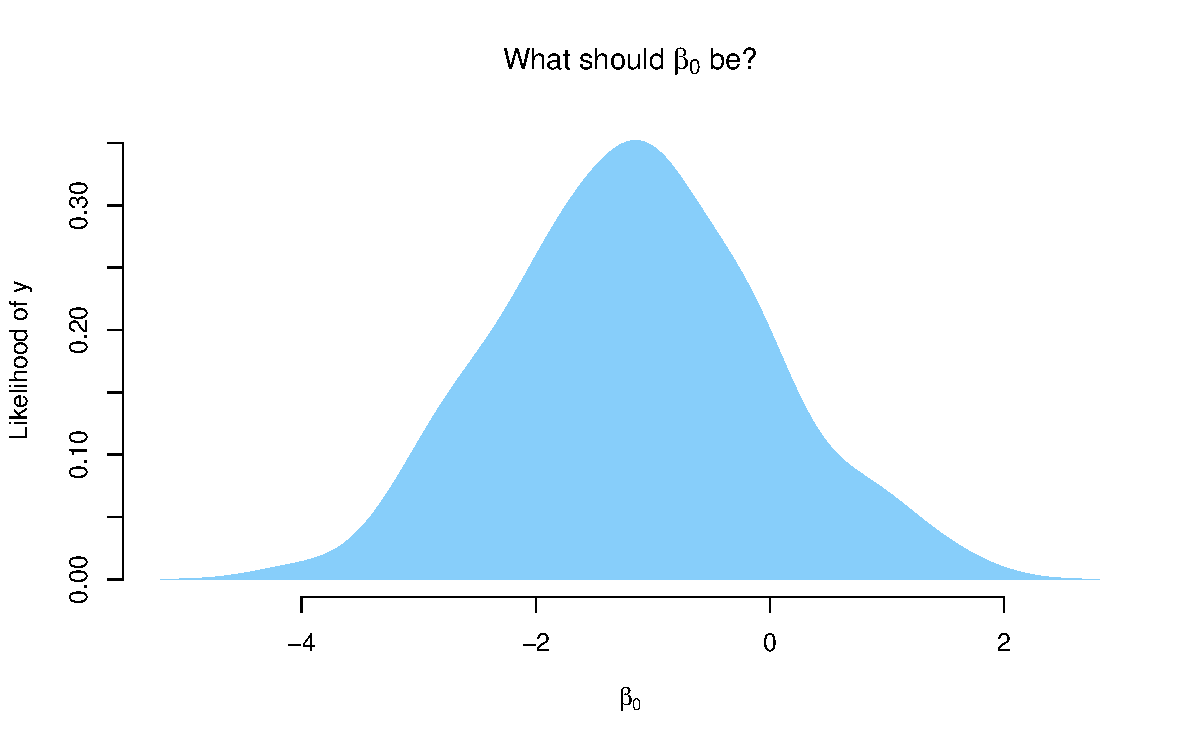
\includegraphics[scale=0.55]{MLE.pdf}
\end{center}

\end{frame}

%@@@@@@@@@@@@@@@@@@@@@@@@@@@@@@@@@@@@@@@@@@@@@@@@@@@@@@
\begin{frame}
\frametitle{Let's return to the Titanic...}

\begin{table}
\begin{tabular}{r | c | c | c | c | c | c | c}
Survived & Pclass  & Name & Sex & Age & Siblings & Parents & Fare\\
 &   &  &  &  & Spouses & Children & \\
\hline \hline
0 & 3 & Owen Harris Braund &M&22&1&0&7.25\\ 
 1 & 1 & Mrs. John Cumings &F&38&1&0&71.28\\ 
  1 & 3 & Miss. Laina Heikkinen &F&26&0&0&7.92\\ 
   1 & 1 & Mrs. Jacques Futrelle &F&35&1&0&53.10\\ 
   $\vdots$ & $\vdots$ & $\vdots$ &$\vdots$&$\vdots$&$\vdots$&$\vdots$&$\vdots$\\ 
%Norman P & 8:00 & 22:45 & 23:02 & 53:47 \onslide<4->\\
%Alex K & 14:00 & 28:00 & n/a & n/a \onslide<5->\\
%Sarah H & 9:22 & 21:10 & 24:03 & 54:35 
\end{tabular}
\end{table}

\end{frame}

%@@@@@@@@@@@@@@@@@@@@@@@@@@@@@@@@@@@@@@@@@@@@@@@@@@@@@@
\begin{frame}
\frametitle{Let's return to the Titanic...}

\begin{center}
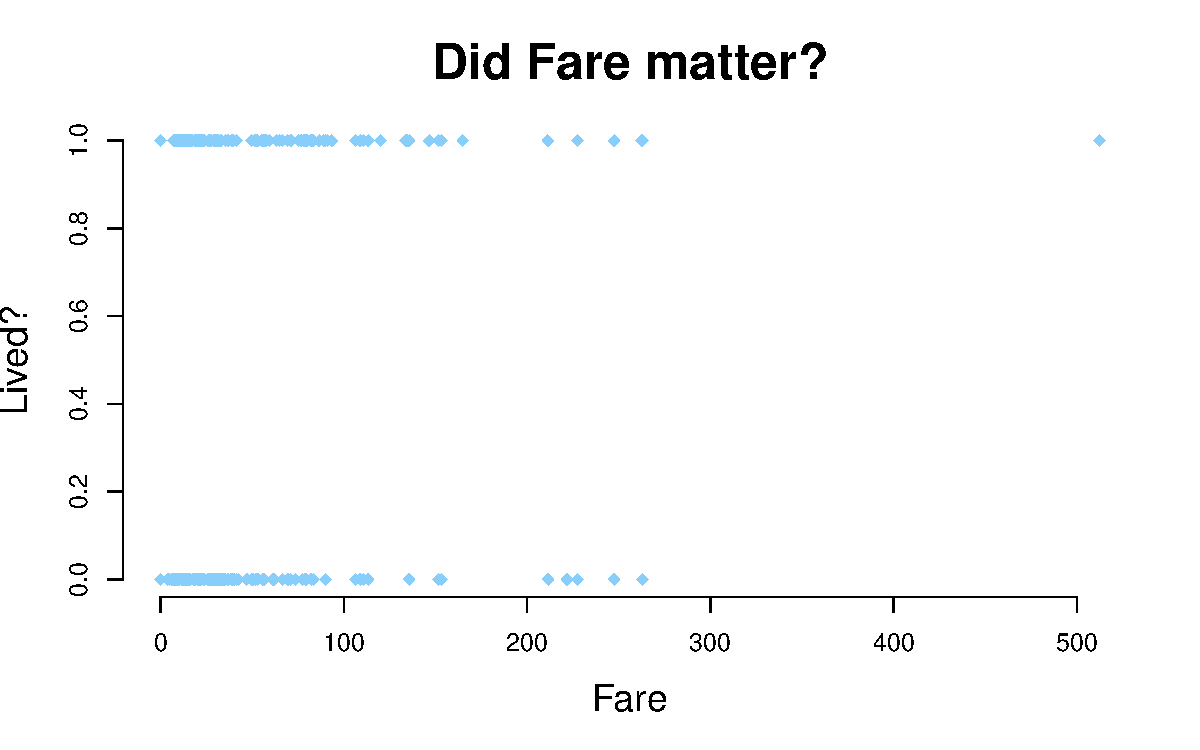
\includegraphics[scale=0.55]{titanic_fare.pdf}
\end{center}

\end{frame}

%@@@@@@@@@@@@@@@@@@@@@@@@@@@@@@@@@@@@@@@@@@@@@@@@@@@@@@
\begin{frame}
\frametitle{Let's return to the Titanic...}

\begin{center}
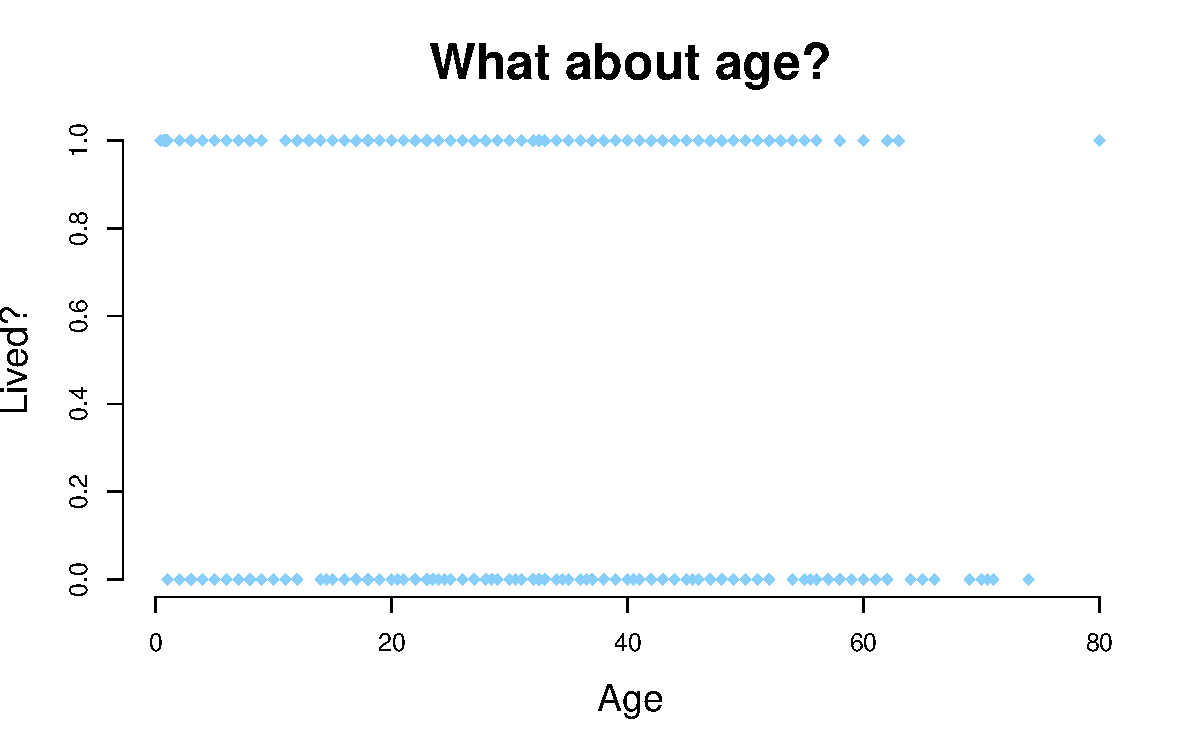
\includegraphics[scale=0.55]{titanic_age.pdf}
\end{center}

\end{frame}

%@@@@@@@@@@@@@@@@@@@@@@@@@@@@@@@@@@@@@@@@@@@@@@@@@@@@@@
\begin{frame}
\frametitle{Let's return to the Titanic... interpret this!}

% latex table generated in R 3.5.1 by xtable 1.8-3 package
% Sun Mar 10 22:01:57 2019
\begin{table}[ht]
\centering
\begin{tabular}{rrrrr}
  \hline
   \hline
 & Estimate & Std. Error & z value & Pr($>$$|$z$|$) \\ 
  \hline
    \hline
(Intercept) & 5.2973 & 0.5574 & 9.50 & 0.0000 \\ 
  Pclass & -1.1777 & 0.1461 & -8.06 & 0.0000 \\ 
  Age & -0.0435 & 0.0077 & -5.63 & 0.0000 \\ 
  Male & -2.7573 & 0.2004 & -13.76 & 0.0000 \\ 
  Siblings/Spouses & -0.4018 & 0.1107 & -3.63 & 0.0003 \\ 
  Parents/Children & -0.1065 & 0.1186 & -0.90 & 0.3691 \\ 
  Fare & 0.0028 & 0.0024 & 1.17 & 0.2437 \\ 
   \hline
     \hline
\end{tabular}
\end{table}

\end{frame}

%@@@@@@@@@@@@@@@@@@@@@@@@@@@@@@@@@@@@@@@@@@@@@@@@@@@@@@
\begin{frame}
\frametitle{Let's return to the Titanic... interpret this!}

So if we were doing linear regression, we would have:
\begin{align*}
y = &\beta_{intercept}\\
 &+ \beta_{Pclass}Pclass\\
 &+ \beta_{Age}Age\\ 
 &+ \beta_{Male}Male\\ 
 &+ \beta_{Siblings/Spouses}Siblings/Spouses\\
 &+ \beta_{Parents/Children}Parents/Children\\
 &+ \beta_{Fare}Fare;\\
\end{align*}
\bigskip
\bigskip
\onslide<2->The effect of Age on $y$ would be just $\beta_{Age}$.
\end{frame}

%@@@@@@@@@@@@@@@@@@@@@@@@@@@@@@@@@@@@@@@@@@@@@@@@@@@@@@
\begin{frame}
\frametitle{Let's return to the Titanic... interpret this!}

Unfortunately, we are doing logit:
\begin{align*}
p(y = \mbox{Lived}) &= \frac{\exp\{\beta_{intercept} + \beta_{Pclass}Pclass + \beta_{Age}Age + ...\}}{1 + \exp\{\beta_{intercept} + \beta_{Pclass}Pclass + \beta_{Age}Age + ...\}};\\
\end{align*}
\bigskip
\bigskip
\onslide<2->The \textbf{effect} of Age on $y$ \textbf{depends on the values for all} the other independent vars!\\
\bigskip
If you want to demonstrate how a variable matters it has to be relative to a particular case:
\begin{itemize}
\item the average or medians of the rest of the variables;
\item a particular substantively interesting case;
\item an observation in the dataset.
\end{itemize}
\end{frame}

%@@@@@@@@@@@@@@@@@@@@@@@@@@@@@@@@@@@@@@@@@@@@@@@@@@@@@@
\begin{frame}
\frametitle{Let's return to the Titanic... interpret this!}

\begin{center}
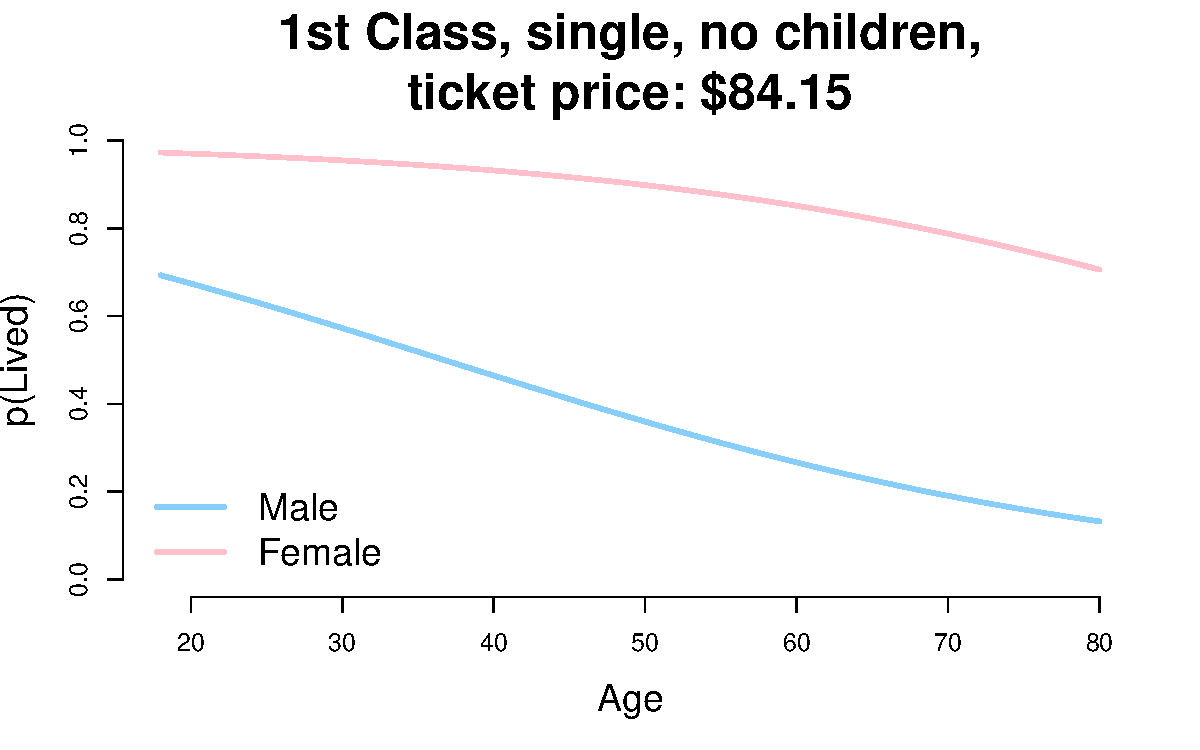
\includegraphics[scale=0.55]{titanic_prediction.pdf}
\end{center}

\end{frame}

%@@@@@@@@@@@@@@@@@@@@@@@@@@@@@@@@@@@@@@@@@@@@@@@@@@@@@@
\begin{frame}
\frametitle{Let's return to the Titanic... interpret this!}

\begin{center}
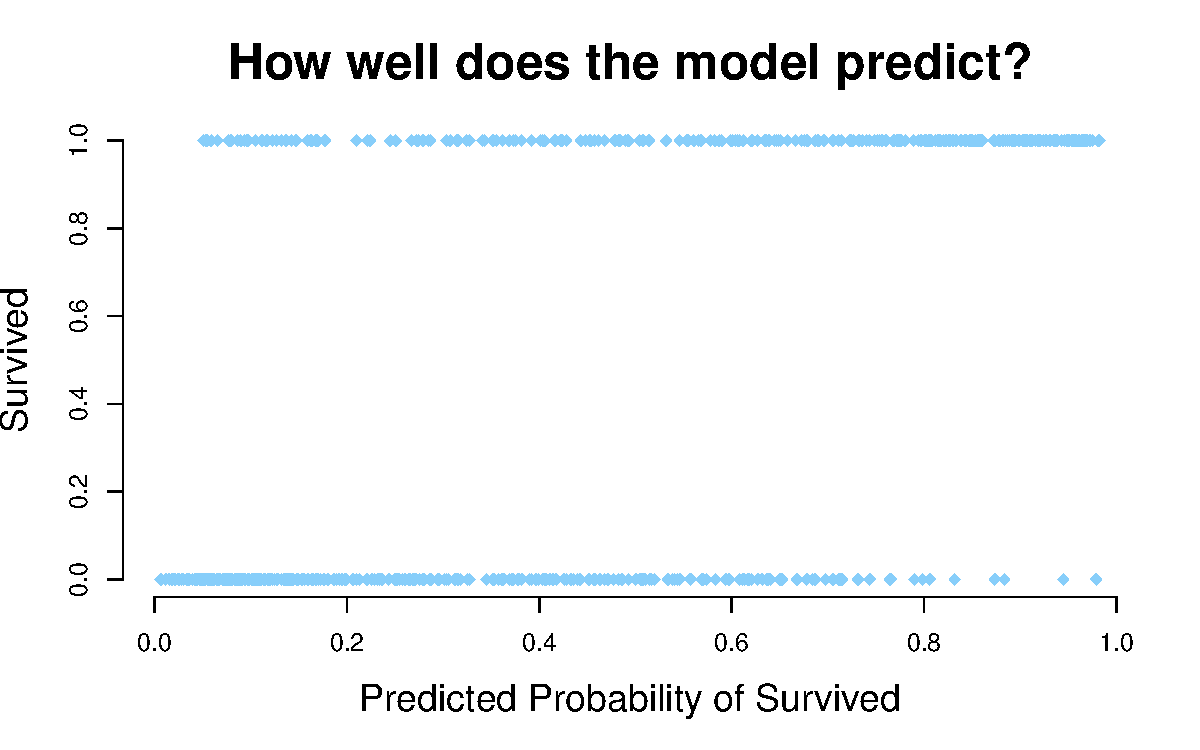
\includegraphics[scale=0.55]{titanic_prediction_data.pdf}
\end{center}

\end{frame}

%@@@@@@@@@@@@@@@@@@@@@@@@@@@@@@@@@@@@@@@@@@@@@@@@@@@@@@
\begin{frame}
\frametitle{Let's return to the Titanic... interpret this!}

\begin{center}
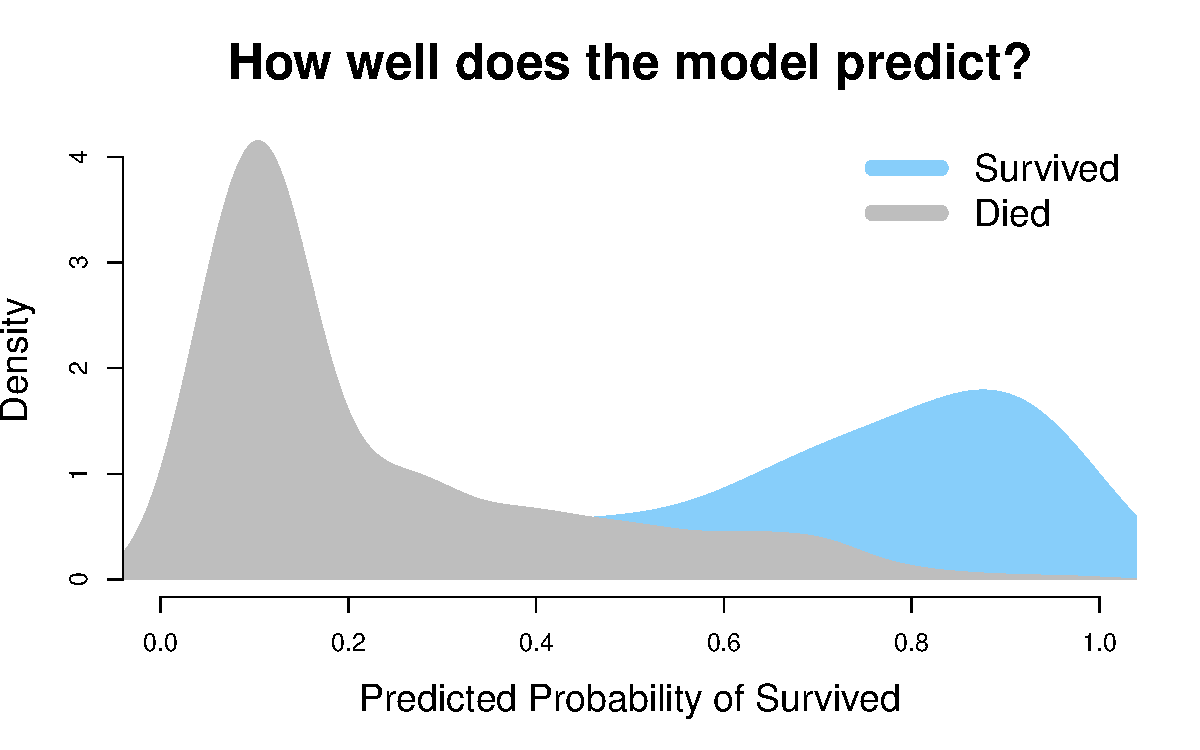
\includegraphics[scale=0.55]{titanic_prediction_dens.pdf}
\end{center}

\end{frame}

%@@@@@@@@@@@@@@@@@@@@@@@@@@@@@@@@@@@@@@@@@@@@@@@@@@@@@@
\begin{frame}
\frametitle{Summary}

Logit is a powerful and ubiquitous method for the relationship between binary dependent variables and numerical or categorical independent variables;\\
\bigskip
\bigskip
Logit is estimated via Maximum Likelihood Estimation;\\
\bigskip
\bigskip
Logit is a GLM - there are tons of GLMs built for different tasks.

\end{frame}










\end{document}

